\documentclass{article}[12]
\usepackage[utf8]{inputenc}
\usepackage{fancyhdr}
\usepackage[margin=2.5cm,twoside]{geometry}
\usepackage[super]{nth}
\usepackage[english]{babel}
\usepackage{csquotes}

\usepackage{hyperref}
\usepackage[backend=biber,style=ieee]{biblatex}
\addbibresource{bibliography.bib}

\usepackage{float}

\pagestyle{fancy}
\fancyhf{}
\fancyhead[LE,RO]{DID - 07 Detailed Design Document (Hebb \& Stephan)}
\fancyhead[LO,RE]{\leftmark}
\fancyfoot[LE,RO]{\thepage}

\usepackage{graphicx}

\begin{document}
	
\begin{titlepage}
	\begin{center}
		\vspace*{1cm}
		
		\LARGE\textsc{Royal Military College of Canada}\normalsize
		
		\vspace{0.2cm}
		
		\textsc{Department of Electrical and Computer Engineering}
		
		\vspace{1.5cm}
		
		
\includegraphics[width=0.3\textwidth]{rmcLogo.png}
		
		\vspace{1.5cm}
		
		\LARGE{Designing \textsc{coatimunde}\\}
		
		\vspace{0.2cm}
		
		\normalsize{Computer Optics Analyzing Trajectories In Mostly Unknown, Navigation Denied Environments}
		
		\vspace{0.1cm}
		
		\normalsize{DID-07 - Detailed Design Document}
		
		\vfill
		
		\textbf{Presented by:}\\Amos Navarre \textsc{Hebb} \& Kara \textsc{Stephan}\\
		\vspace{0.8cm}
		\textbf{Presented to:}\\Dr. Sidney \textsc{Givigi} \& Capt Anthony \textsc{Marasco} 
		\vspace{0.8cm}
		
		\today
		
	\end{center}
\end{titlepage}

\pagenumbering{roman}

\section*{Acknowledgement}

We would like to thank our supervisor, Dr. Sidney Givigi, for first introducing us to the problem of real time obstacle avoidance and providing us access to the tools and robots we used to complete our work.

\section*{Abstract}

The C\textsc{coatimunde} project attempts to extract target and depth information from a single camera feed source using the Robot Operating System as both an underlying architecture and a design philosophy. Four custom `nodes' are created which interact with existing nodes necessary to execute Robot Operating System code. These nodes identify targets, identify depth information, record movement of the robot, and compile it into a single set of points which allow the program to send appropriate commands to the robot to navigate toward targets while avoiding obstacles.
	
\tableofcontents \newpage

\pagenumbering{arabic}


\section{Introduction}

	\subsection{Document Purpose}
	
	Using Computer Optics for Analyzing Trajectories in Mostly Unknown, Navigation Denied, Environments (\textsc{coatimunde}) is the goal of this project. The purpose of this document is to outline the detailed design for \textsc{coatimunde}, including any deviations from the Preliminary Design Specification, what the final design is, how it was built, and how this met the requirements of the project, as specified in the Statement of Requirements. 
This design of the project is shown, through design artifacts, and discussed in the section 2. Section 3 provides equipment information for the project. Section 4 presents the verification and validation for each component of the project, some of which produced images like those shown in Figure \ref{fig:prettyresultsimage}. The final results of the project are presented in section 5. Section 6 then provides a discussion of the degree of success of the project and provide feedback on the course experience as a whole in.
	
	\begin{figure}[]
		\centering
		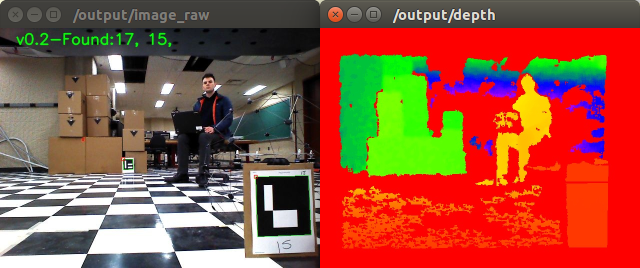
\includegraphics[width=0.95\linewidth]{results}
		\caption{Visual Output of Running \textsc{coatimunde} Software}
		\label{fig:prettyresultsimage}
	\end{figure}
	
	\subsection{Background}
	
	The use of autonomous aerial vehicles is growing quickly, both in the consumer and professional sectors. Currently these vehicles rely on skilled pilots to accomplish a very limited set of tasks. Adding obstacle avoidance capabilities to these vehicles and simplifying the task of following targets could greatly expand the utility of these vehicles and allow for them to be used in many more situations. This section gives a quick background on obstacle avoidance, unmanned aircraft systems, computer vision, and the platforms we intend to use in this project.

		\subsubsection{Aim}
	
		The aim of this project is to design a high level control system that will allow an air robot to identify a target and move towards it, avoiding any obstacles that are in the way. The ultimate goal of this project is tracking targets of interest in complex environments with a flying robot. To accomplish this goal a TurtleBot and then a flying robot are used with only the use of a single camera to identify targets and obstacles. 
		
		\subsubsection{Benefits}
		
		Having a flying robot capable of accomplishing the desired tasks while remaining totally autonomous will hopefully translate into improved performance from flying robots in environments closer to the ground, and will assist pilots in complex environments. These general requirements can be used in many situations. These potential benefits to society as a whole are the motivation behind this project. The following are the benefits for this project :
		\begin{itemize}
			\item \textbf{Surveillance:} The robot could follow an interesting object, especially in an urban environment, without colliding with obstacles.
			\item \textbf{Search and Rescue:} The robot could assist in search efforts by moving towards visual way-points set by pilots while avoiding obstacles in complex environments.
			\item \textbf{Inspections:} The robot could inspect objects in hard to reach and complex environments like rooftops or bridges.
			\item \textbf{Disaster Relief:} The robot could check inside of buildings that may have compromised structural integrity, rubble on ground, etc.
			\item \textbf{Agriculture:} The robot could inspect tree-fruit or crops that cannot be observed from overhead and it could check assets in remote locations such as irrigation equipment.
		\end{itemize}

		\subsubsection{Scope}
	
		The project started through the use of a ground robot and then progressing to a flying robot. The project used computer vision to find targets and for avoiding multiple obstacles. Both robots are highly autonomous, requiring only user input to commence. 

		The scope of the project was limited due to being restricted to testing indoors. Ideally the unmanned aerial vehicle (UAV) would be operating at a high speed and identifying an arbitrary target in an unpredictable environment. In this case, the testing was completed within the confines of a relatively small robotics laboratory. Smaller obstacles were used indoors simply due to space constraints. Lower speeds were used as well, again due to the lack of space. 


		\subsubsection{Requirements}
		
		The requirements for the project are described in the Statement of Requirements (DID-03) \cite{sor}. The main functional requirements for this project were identification and movement towards a target within 15m radius and identification and avoidance of multiple obstacles. 
	
		The initial requirements show certain assumptions that were made which can be attributed to ignorance at the time. The most notable of these is the use of a single video stream and exclusively OpenCV to parse depth data. It proved very difficult to extract reliable depth information from a single camera. Although initially a method using stereo cameras had been identified, the push-broom approach \cite{barry2015pushbroom} had been explored, it was abandoned due to a belief that depth from a single camera would be similarly visible, and thus constrained ourselves in the requirements phase to this.

		\subsubsection{Preliminary Design}
		
		The preliminary design document outlines the initial design for the project \cite{pdd}. The initial design was fairly robust, but certain aspects had intentionally not yet been selected. The main block diagram Figure \ref{fig:blockdiagram} remains unchanged, the only additions are the specific topics being subscribed to by each of the custom modules. 
		
		The most substantial changes came to the actual actions to be performed by each node. Given that the nodes were intentionally left fairly undefined and only their specific input and output were described, this allowed for fairly substantial changes to the underlying logic that allows these nodes to complete their tasks.


This initial design has been changed since the document was presented. It was modified as unforeseen problems with the design came to light and deviations were made to ensure the project was meeting the requirements.


		\subsubsection{Changes to Schedule}
	
	While Robot Operating System (ROS) is a very flexible framework for writing robot software, there was a significant understanding of the underlying plumbing needed before some of the higher level capabilities could be used. Most of the changes to the schedule are a result of over-estimating how difficult it would be to implement some of the higher level aspects of this project, and significantly under-estimating how much time it would take to do simpler tasks.
	
		\subsubsection{Changes to Custom Nodes}
	
	Rather than using a pre-existing set of nodes, custom nodes were created in accordance with the preliminary design. The most notable changes are only in what specific information was passed between different nodes, in particular the way that depth information was parsed from a registered depth image. By parsing all information from a single depth image and including information about ArUco marker locations instead of attempting to use other mechanisms, the intent was that on the flying platform, this information could be extracted in exactly the same way once a mechanism to extract depth information from a single camera image was developed.
	
	\subsubsection{Porting to UAV}
	
	Presumably delayed forever, the inertia to simply make this execute on a platform that allows very reliable feedback and predictable reactions to inputs means that, given our lack of exposure to the flying platform, it is not implemented in its final form on a flying platform. 

	\subsection{Definitions}
	
		\subsubsection{Obstacle Avoidance}
		
		Obstacle avoidance is the task of satisfying a control objective, in this case moving toward a visual target, while subject to non-intersection or non-collision position constraints. The latter constraints are, in this case, to be dynamically created while moving in a reactive manner, instead of being pre-computed.
		
		\subsubsection{Unmanned Aircraft Systems}
		
		Very generally, any powered vehicle that uses aerodynamic forces to provide lift, without a human operator being carried, can be considered an unmanned aerial vehicle. Currently most of these vehicles make up a single component of a larger unmanned aircraft system. An Unmanned aircraft system (UAS), or remotely piloted aircraft system (RPAS), is an aircraft without a human pilot on-board, instead controlled by an operator on the ground. Such a system can have varying levels of autonomy, something as simple as a model aircraft could be considered a UAS without any automation capabilities.\cite{RPAS}
		
		\subsubsection{Computer Vision}
		
		Currently there are many different ways that computers can make high-level decisions based on digital image information. There are many methods to acquire, process, and analyze data from the real world using a camera. While this is a very broad field, the intended focus is on motion estimation and object recognition, using a video stream taken from a camera. 
		
		Motion estimation can be accomplished using direct methods which compare whole fields of pixels to each other over successive frames, compared to other indirect methods which look for specific features. The information resulting from motion estimation streams can be used to both compensate for motion while analyzing other aspects of an image, and to update a state machine.
		
		Object recognition in our project will accomplish two tasks: identifying a marker or target which will require more involved object recognition calculations, and very simple techniques, such as edge detection, identifying obstacles that exist in the path of the robot.
		
		\subsubsection{OpenCV}
		
		The Open Source Computer Vision Library (OpenCV) of programming functions is a cross-platform and free for use collection of functions primarily aimed at real-time computer vision\cite{opencv}. Most well documented techniques to accomplish all of the computer vision goals of our project have already been created and refined in OpenCV.\cite{woods2015dynamic} For this reason this project utilized many preexisting OpenCV functions.
		
		\subsubsection{Gazebo}
		
		Gazebo is a robot simulator that allows for the creation of a realistic environment which includes both obstacles and markers similar to those being used in the laboratory testing environment. It was then used to rapidly test algorithms.
		
		\subsubsection{Robot Operating System}
		
		The Robot Operating System (ROS) is a distributed message system that allows for various sensors and processors to work together to control a robot. It is open source and has been integrated already with OpenCV and Gazebo. There are many additional tools for detecting obstacles, mapping the environment, planning paths, and much more. ROS is also a robust messaging system that has been proven to be capable of real-time processes.
		
		\subsubsection{gmapping}
		
		OpenSLAM has developed gmapping to create grid maps from laser range data. It uses a Rao-Blackwellized particle filter where each particle carries an individual map of the environment. Then the number of particles needed are reduced to create a more accurate map with significantly reduced uncertainty.\cite{grisetti_stachniss_burgard}
		
		While this process relies on laser information, and it is only ever used in its unmodified form for this project, the intent was to port it, so it would work with a slice from a depth registered image. This would allow it to work on a platform with only a single camera, a process that has been shown to turn a three-dimensional field into a two-dimensional map accurately.\cite{2018nanomap}
		
		
		\subsubsection{TurtleBot}
		
		The TurtleBot is a robot kit with open-source design and software. It is built to the specification for TurtleBot Compatible Platforms\cite{wise_foote_2011}. In this case the TurtleBot has a Kobuki Base, an Acer Netbook running Ubuntu with ROS packages added, an X-Box Kinect, and some mounting plates. 
		
		The resulting robot looks like a disk supporting some circular shelves with a small laptop and a camera on the shelves. The base disk is 35.4cm in diameter, the topmost shelf is 42cm from the ground. The robot has a maximum speed of 0.65m/s. 
		
		\subsubsection{AscTec Pelican}
		
		The Ascending Technologies Pelican is a 65.1cm by 65.1cm quad-copter designed for research purposes\cite{asctec}. It includes a camera, a high level and low level processor set up for computer vision, and simultaneous localization and mapping (SLAM) research. It is also capable of interfacing easily with other controllers and can carry up to a kilogram of additional gear. This particular flying robot comes installed with a single camera, that was used to collect stereo data and was later used for depth information.

		
\section{Design}
	
	\subsection{Computer Vision}
	
	Computer vision as defined prior is acquiring, processing, and analyzing data from the real world using a camera. Computer vision identifies objects in the surrounding environment, specifically targets and obstacles. Computer vision was used as an input source for this project in seven unique manners; these are target finding,obstacle finding, pinhole camera, depth registered image, stereo depth estimation, amcl, and RViz. Computer vision was also attempted with optical flow but that was found to be out of the scope for the project. The implementation of these created a navigation kit that exclusively uses a camera as input, resulting in a very transferable and lightweight package for flying robots. Computer vision using a single camera is also a constraint of the design as laid out by the SOR \cite{sor}.

		\subsubsection{Target Finding}
		
		While finding arbitrary targets is preferable, this project is limited to finding special targets designed to be easily identified in a busy environment. These targets are called ArUco shapes. There are existing libraries in OpenCV that are useful for identifying ArUco shapes with very little overhead. The identification of the targets was done through computer vision and extracting the key features from these markers. 
		
		\subsubsection{Obstacle Finding}
		
		Finding obstacles is a considerable aspect of this project. There are various algorithms which leverage the robot's motion through the environment to extract key features of the environment, indicating the potential presence of obstacles. Parallax shift is the tendency for items that are closer to a camera to appear to move more or change in size more than a background that is further away. This shift can be used to indicate where items are and how close they are. Occlusion is where one item moves in front of another item and covers it up. When this occurs it indicates that the item still in view is closer to the camera than the item that has been hidden. OpenCV contains libraries for both of these tasks, as well as others that may end up being employed to identify obstacles in the environment.
		
		\subsubsection{Optical Flow}
		
		Optical Flow is a possible source of motion information for the robot. As a camera is moved through an environment, the entire image will appear to scale larger as the camera moves forward, rotate left and right as a robot rolls, and shift left, right, up, and down as the robot pitches and yaws. Calculating shifts from one frame to another for global shifts caused by movement of the camera is a mathematically intensive process beyond the scope of this project. OpenCV contains libraries to try to parse this information, but it requires a considerable amount of effort to combine this information with a model of a robot to get useful position estimation. Given the extreme difficulty of extracting meaningful information from a camera, especially given the very constrained geometry of a single camera, means that this approach is not used in this project.
		
		\subsubsection{Pinhole Camera}
		
		The pinhole camera, in this context, is not an existing camera, but a mathematical construct which models the relationship between objects in three-dimensional space, and a projection onto an image plane. Images are grids of pixels, and ideally a straight line from any point on this grid, through a single point in front of the plane, would terminate at the real location in three-dimensional space of the object in the photo. Real cameras use lenses and imperfect capture devices which introduce distortion. This is ignored for the most part, and only objects in the centre of the camera's field of vision are used in this project, this is computationally inexpensive and allows software to be ported between different cameras quickly. 
		
		\subsubsection{Depth Registered Image}

A depth registered image is one where pixels hold an extra value. This value is a distance in real space at a known scale. This allows for distances to targets and interesting points to be easily extracted from the image. These can be created in hardware using advanced sensors like the Astra Pro on the TurtleBot 2, or using other post-processing techniques. Depth registered images are essential in determining depth information for targets and obstacles in the project. When key features of a target or obstacle is found the depth registered image is parsed to identify the location of these features. This information is then used in the path finder node to determine the robots movement towards the target.   
		
		\subsubsection{Stereo Depth Estimation}
		
		By using two vantage points, depth information can be extracted by examining interesting points in the two vantage panels. Several pre-processing steps are required for this technique to be most effective, all of which are built in to OpenCV. Undoing distortion caused by cameras allows comparisons to be made between images and a three dimensional image to be rectified. This rectified image can be corrected using a known scale, then mapped back to one of the input images, creating a depth-registered image. The correction of distorted images is important as it ensures the depths read from the depth registered image are correct. As depth registered images are necessary for the project ensuring the values in these images is imperative.
		
		\subsubsection{amcl}
		
		amcl is a probabilistic localization system for a robot moving in two dimensional space. Using adaptive Monte Carlo localization \cite{doucet_freitas_gordon_2001} it is able to quickly estimate the pose of a robot against a known two dimensional map. It is implemented as an already existing node in the standard ROS navigation stack, a stack containing code related to finding where the robot is and how it can get somewhere else.
		
		\subsubsection{RViz}
		
		\begin{figure}[]
			\centering
			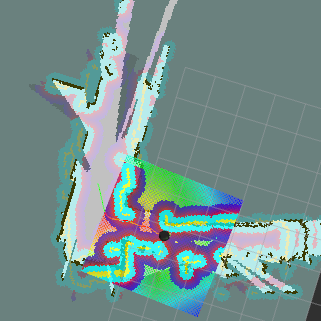
\includegraphics[width=0.5\linewidth]{rviz_screenshot}
			\caption{RViz Visualization of amcl Localization in Angled Hallway}
			\label{fig:rviz}
		\end{figure}
		
		RViz is a visualization tool for ROS, it contains many tools to observe output from various ROS topics. Most notably, there are mechanisms that allow for the visualization of the amcl mapping and goal finding processes showing the robot is a point navigating a two dimensional birds-eye-view of what it perceives its environment looks like. An example of typical RViz output while running amcl is seen in Figure \ref{fig:rviz}.
	
	\subsection{Analyzing Trajectories}
	
	Analyzing trajectories is a term that refers to the robot completing movements towards the target.
To do path planning, the project will implement potential fields. With potential fields, a robot perceives an attractive or repulsive force (represented by vectors) originating from objects in the environment. The robot achieves the required behaviour by appropriately  reacting to these forces, expressed a single resulting force vector that is the sum of all perceived forces \cite{hwang1992potential}.
The use of potential fields allows for the path finding node to decide what movement, in the moment, is best to get closer to the target and further from obstacles.  
 
This algorithm was selected to do path planning as the robot will not have to build a map of the environment to create path to the target \cite{bortoff2000path}. Potential fields allow for the robot to change its path along the way if it discovers new obstacles. This approach to movement does not require complete knowledge of the environment it is navigating. In its simplest implementation the environment must be sparsely populated with obstacles, or simple things like straight lines can become `wall traps' and a robot can become impossibly lost.

	\subsection{Obstacle Avoidance}
	
	There are multiple approaches to obstacle avoidance. The simplest require no prior knowledge of the environment they are navigating and simply react to obstacles as they appear. This approach can be useful for high-speed applications with sparse obstacles, \cite{barry2018high} but become more limited in smaller spaces.
	
	Using more complex algorithms that require more knowledge of the environment end up being easier when a complete map is saved. For this project the amcl localization system is used, which relies on a known map and fairly simple path planning algorithms which are able to solve more complex routes, at the expense of needing to spend more time estimating the robots position in the environment.\cite{doucet_freitas_gordon_2001}

	\subsection{Unknown and Navigation Denied Environments}

	The robot must always remember where identified targets and obstacles are in relation to itself even when its own position changes. Navigation denied means that the robot does not have access to a GPS to locate itself, so it must search its unknown environment to identify targets and obstacles. An unknown environment can be defined as an environment in which the robot has no prior knowledge of its surroundings and must identify objects in this environment itself through computer vision. 
Target and obstacles are recorded and their vectors are updated in the potential fields to track the locations of each object. These vectors are used in the state machine to properly create a path to the target, as they are either negative for the target or positive for obstacles. This is the reason that the project is using potential fields to be able to plan the path to the target. 


	\subsection{Architecture}
	
	The architecture of \textsc{coatimunde} can be seen in Figure \ref{fig:blockdiagram}. It is a very high level overview and does not contain references to most of the hardware in use for a main reason, the actual robot and laptop being used are relatively arbitrary as long as the software included is present on both. ROS also includes many nodes which are not represented on the block diagram. Only the nodes that are most important to our project have been specifically added to ROS, or have been custom created are included on our system block diagram.
	
	The laptop contains the initialization, target selection, and RViz. The laptop also takes the user input when necessary and processes it appropriately.  The robot does all the target identification, obstacle avoidance, and movement decisions autonomously. This means it takes the input from the camera into a video processing node and then creates a corresponding ROS message to be sent to the other systems on the robot. These messages are created and used throughout the different systems on the robot. The model of the robot's environment is found through subscribing to messages from the obstacle finder node, target finder node, and the state estimate node. This model then creates a message to pass to the route planning node which tells the movement node how to update its position and speed. 
	
	Most of the nodes used in this project are either being used stock, or are very minimally modified from provided libraries. The four nodes, highlighted in grey, which have been custom built for this project are the State Estimate, Target Finder, Obstacle Finder, and Route Planner. Along with each of these functional names assigned, the actual nodal name for each of the project's custom nodes are listed.

	\begin{figure}[H]
		\centering
		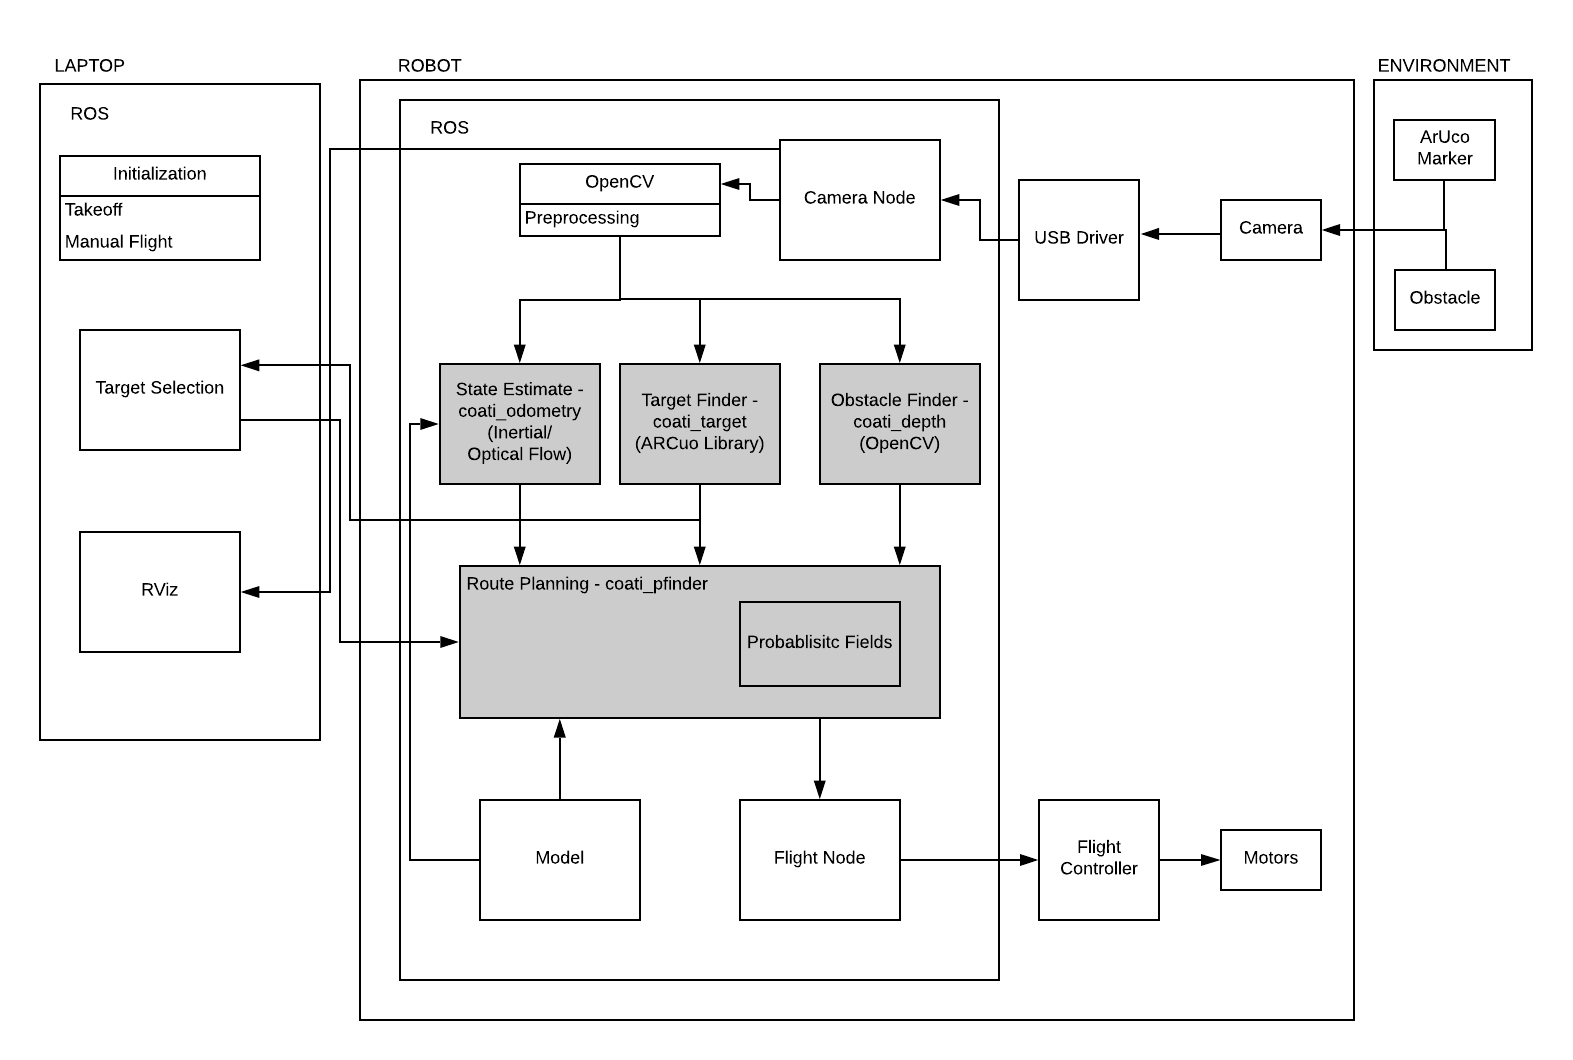
\includegraphics[width=\linewidth]{BlockDiagram}
		\caption{Project Block Diagram}
		\label{fig:blockdiagram}
	\end{figure}

	\subsection{Custom Nodes}
	
 All of the nodes written for this project are written in Python and then built in ROS to be implemented on the robot. Python is used for this project because C++ and Python are the most supported languages for both ROS Nodes and OpenCV. While C++ could possibly be faster in execution, most of our bottlenecks occur from the actual processing of images. The library calls to OpenCV are still executing in the lower level C that OpenCV was written in, so there would be minimal gains had we written it in C++.
 
 The Camera node is referenced in many locations. The camera node is built into ROS and provides image data in various formats. Processes can subscribe to these different image formats. In general the raw image information is used by some of the custom nodes and many other built in nodes. Common transformations that must be applied to all photographs was added to the camera node. These transformations are to correct for the distortion that any camera has due to its own geometry.
	
	\subsubsection{Target Finding}
	
	\begin{figure}[H]
		\centering
		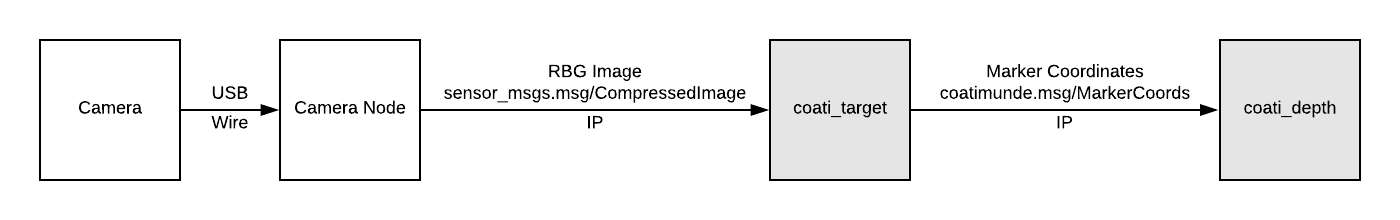
\includegraphics[width=0.9\linewidth]{TargetDiagram.png}
		\caption{Target Finding Node}
		\label{fig:target}
	\end{figure}

	Camera data, after being processed by the camera node, goes into the target finder node. The target finder is mostly implementing the ArUco symbol finding libraries in OpenCV passing messages as shown in Figure \ref{fig:target}. ArUco symbols are intended for augmented reality purposes and provide very accurate position, orientation, and distance information. These values are inserted into a marker coordinate message that the other systems on the robot can understand and be published at least ten times per second.
	
	Given the limited field of view of the robot, it cannot always be able to see the target. The robot, in the pfinder node, saves a dictionary of points that are associated with targets that have been resolved. Only the most recent `citing' of a target is recorded, and as soon as odometry updates are provided about the location of a target the last known location is updated with these transformations.
	
	\subsubsection{Obstacle Finding}
	
	\begin{figure}[H]
		\centering
		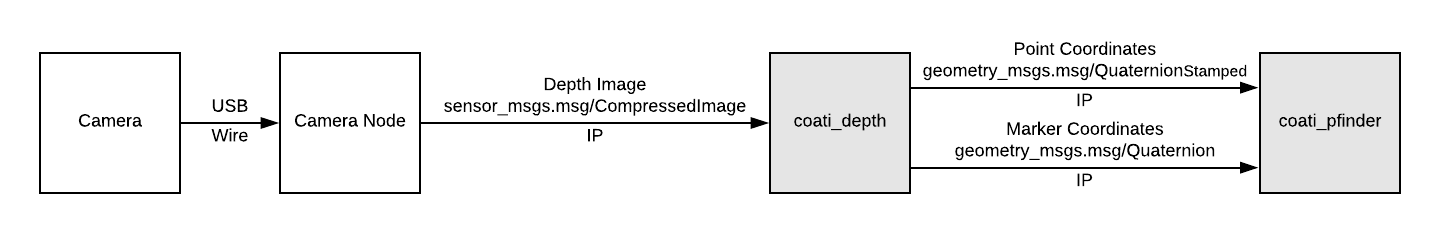
\includegraphics[width=0.9\linewidth]{DepthDiagram.png}
		\caption{Obstacle Finding Node}
		\label{fig:obstacle}
	\end{figure}

	Finding obstacles with depth information is difficult using monocular vision. The approach currently is to take advantage of the efficiency of the quaternion math allowing the finder node to update many points at once, and to sample many points along a plane at all times. When an image is processed, the depths along a row of pixels through the center of the image are converted into depth vectors which are published constantly according to the block diagram shown in Figure \ref{fig:obstacle}. 
	
	Getting depth information from a single camera is still a topic of ongoing research to which there are no simple existing solutions. The TurtleBot also has a suite of depth sensors built in with the camera so these may be used initially instead of trying to use parallax information from a camera to allow for testing other aspects of the system. Currently the approach, which does not work on the flying platform with simpler cameras, is to combine the depth information from another sensor with the image information, and then to sample depths from this.
	
	A node should be created which uses the results from a convolutional neural network trained to extract depth information from images to create a similarly depth registered image file with the camera on the flying platform from a single camera source.
	
	Targets, extracted from the images as well, report the depth to a point exactly in the centre of the target, and the same geometry used to calculate angles away on a camera is used to calculate where the vector to the target should be recorded. All targets are assumed to be in an even plane to the robot, so any x or y rotations are ignored, and it is assumed that targets only have z rotations and absolute distances. The current program, lacking a non-distorted image, only registers new targets that are in the centre of the camera range, and assumes that they are straight ahead.
 
 	The depth node subscribes to the target node to get the target locations. The depth node then uses the given location to find the depth value for the target. This target depth value is transformed in a quaternion and passed off to the path finder node. 
 
 \subsubsection{Limitations of Obstacle Finding Approach}
 
 This approach proved sufficient in the lab environment, but is not very robust in larger environments and leaves the robot in a very reactive state. By not attempting to group together vectors which all point to a single obstacle, the robot is unable to navigate through many simple configurations of multiple obstacles, and never has any memory of an obstacle once it had passed it. 
 
 Error accumulation is also significantly faster for this reason, points would all diverge resulting in obstacles appearing larger and larger the longer the robot drove toward them. If instead an approach where the geometry of the obstacle is worked out and fixed-sized boxes were used internally to model obstacles, they would presumably not diverge in the same manner. 
	
	\subsubsection{State Estimator}
	
	\begin{figure}[H]
		\centering
		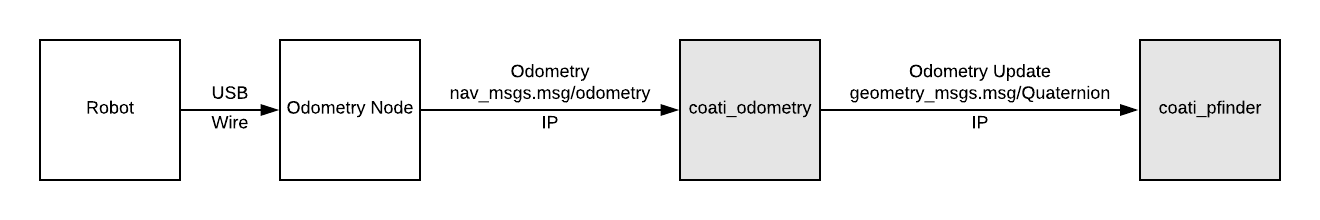
\includegraphics[width=0.9\linewidth]{OdometryDigram.png}
		\caption{State Estimating Node}
		\label{fig:state}
	\end{figure}

	State estimating from camera information is very difficult and computationally expensive. The TurtleBot has stepper motors that can measure distances fairly reliably, and the Quadcopter has accelerometers that provide changes in position more reliably than image information could. 
	
	Even given these fairly reliable sources of odometry, error in the robots knowledge of its location in the environment were shockingly error prone. The need for location estimation beyond dead reckoning is required, however, this was outside the scope of the project.
	
	Creation of a reliable system to extract pose information from camera information is well beyond the scope of this project.
	
	These simpler forms of measuring the robot moving through the environment are used and the odometry node subscribed to the robot's odometry updates, according to Figure \ref{fig:state}. This node turns all state updates into quaternions and publishes them for the route planner. The route planning node then adjusts the vectors to nearby obstacles and targets according to how much the robot has moved. 
	
	New position estimates are provided at least 10 times every second in the form of a quaternion from the last position that the robot was in passed over a ROS message.
	

	\subsubsection{Route Planning}
	
	\begin{figure}[H]
		\centering
		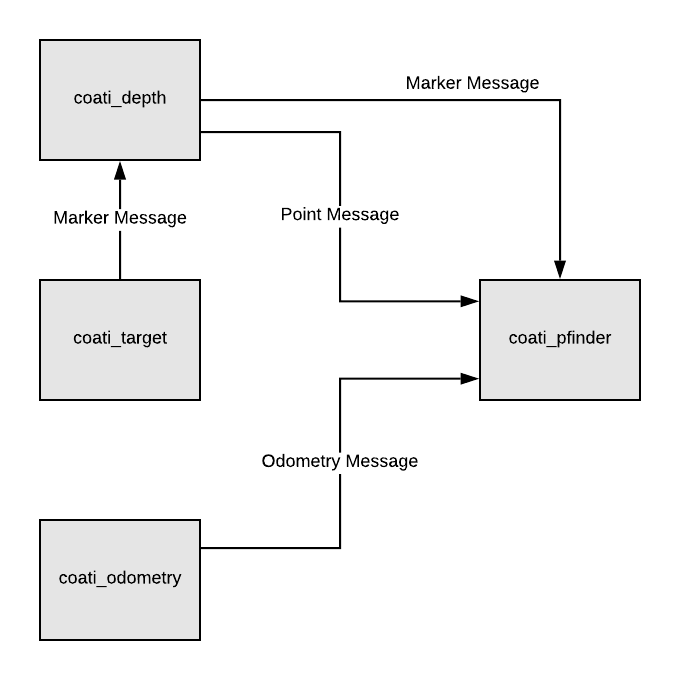
\includegraphics[width=0.6\linewidth]{PathFinderDiagram.png}
		\caption{Route Planning Node}
		\label{fig:routeplanning}
	\end{figure}

	Route planning takes input from the other three custom nodes and determines a route that should carry it toward the target as shown in Figure \ref{fig:routeplanning}. The implemented solution was to create a potential field where positive vectors that repel the robot are attached to all obstacles while a large negative vector is attached to the target location.
	
	As the route node receives more information about the robot moving through the environment it applies transformations to all of the contained vectors to keep them up to date with where they are as the robot changes position in the environment. 
	
 Target locations are all stored in a separate array to remember the location of every target the robot finds. Differentiating targets is simple as each ArUco marker has an associated identification value. These values allow the node to know when a target has been re-spotted and over-write it or allow for finding and remembering the positions of multiple targets. If it discovers a new target it simply adds it to the array with its positional information.
 
 	\subsubsection{PFinder v1}
 
 	The first path finding method is a very simplistic and totally linear attempt at using a potential field system. Vectors toward all points in space, including obstacles, goals, and walls, were constantly updated and the robot would attempt to centre itself along the vector pointing toward the goal, while all other vectors are only avoided when dangerously close.
 
 	Error accumulation resulted in two things, the robot failing to reach the goals as soon as it was too close to capture the entire ArUco marker, meaning that effectively it still required line-of-sight, and all obstacles appear dangerously close often after very little movement in their general direction. 


	The method to remove unnecessary or repetitive vectors for obstacles is to have these vectors simply expire after a certain amount of time. This amount of time, to be platform independent, is not a set value, but instead is based on the requirement to provide a new update 10 times every second. If, when applying transformations to all stored vectors, the node requires more than 0.1 seconds to execute, it deletes the oldest half of the nodes it is aware of. This continuous addition and replacement system ensures that large numbers of points can be remembered, while ensuring that performance requirements are met.
	
	\subsubsection{PFinder v2}
	
	The navigation suite for ROS comes with many tools for more accurate state estimation. The biggest problem with PFinder v1 is the rate at which errors accumulate, making any attempts to navigate with the ground robot unsuccessful, and estimations on the flying robot are totally useless.
	
	The most interesting tool for our purposes is amcl. amcl is a localization system for robots moving in two dimensional planes. According to our scope both the TurtleBot and the flying robot should be able to do this using a very simple particle filter to track the pose of a robot. While this approach to probabilistic localization is the simplest, and therefore easiest to understand, it also relies heavily on a known map, something our project definition does not allow.
	
	In a small lab environment with a fairly high density of objects, slower but more accurate movement is desirable. So the decision to quickly develop a map and then try to navigate this was made. GMapping was used to create a map on startup, and then amcl would be used to navigate this newly created map. New maps could be created any time the robot became lost, allowing for the use of very short-ranged sensors and to enable navigation of a mostly unknown environment.
	
	The PFinder v2 first rotates in place while running the gmapping node and records the locations in real space of all of the ArUco markers that are discovered using the existing output. These points are then stored in an array relative to the absolute position of a fixed marker, defined arbitrarily by the gmapping node. At the same time, gmapping is creating a map using laser depth information from the Astra Pro, although the intention is to modify this behaviour to allow it to record information from the depth-registered image the depth node is still generating from the camera output.
	
	Once a full rotation has been performed, the amcl node is launched, and PFinder provides a user with targets to select from. Once a user has selected a target for the robot to navigate toward its absolute location is passed into the \texttt{/move\_base\_simple/goal} topic as a goal to which ROS has existing logic to navigate toward. Solving the navigation to this goal is achieved using both the map created initially, overlaid with any currently occupied areas discovered by amcl. amcl naturally updates these locations based on current laser data, and removes them if an obstacle is removed. This allows for the robot to make very accurate decisions while avoiding obstacles in real time. 
	
	\subsection{Node Diagram}

	\begin{figure}[H]
		\centering
		\includegraphics[width=0.8\linewidth]{NodeDiagram}
		\caption{Project Node Diagram}
		\label{fig:nodediagram}
	\end{figure}


	All nodes created or used in the project are shown in Figure \ref{fig:nodediagram}. The diagram illustrates what node subscribes to the other nodes, such as the target finder node subscribes to the camera node to get messages about the target's potential location. 
	
 	It is important to recognize that the directions indicated in Figure \ref{fig:nodediagram} are the flow of messages, not the direction of the subscriptions. 

	\subsection{Mathematical Modeling}
	
		\subsubsection{Flying Robot}
	
		Given that a quad-copter has six degrees of freedom, modeling them is a very difficult task. The AscTec Pelican already has many existing models intended for use with ROS. There is also a large collection of hardware agnostic tools for operating a quad-copter.
	
		\subsubsection{Initial Approach to Robot in 3D Space}
		
		The robot itself needs to remember where it is located in its environment. Remembering where targets are located relative to the robot is necessary, and presumably remembering the locations of obstacles are used as well. Using quaternion vectors relative to the robot allows for simple transformations on these vectors while using very little computational power \cite{williams2010combining}. ROS contains methods and messages to easily communicate, convert, and apply transformations to quaternions.
		
		The limitations to this approach are the limited accuracy of the very small quaternions that result from real time odometry information from the robot, and the rate at which error accumulates when blindly trusting all robot odometry. 
		
		To combine two vectors, they are multiplied together. The result is a very accurate representation when both vectors are quite accurate and are similar in size, but when repeatedly multiplying a very small vector with a larger vector the errors compound very quickly and points diverge and become useless far faster than anticipated.
	
		\subsubsection{Pose Estimation}
	
		Initially feedback from inertial sensors is used for pose estimation, but ideally a version of Optical Flow is used to estimate the position of the robot in 3D space. There are some libraries in OpenCV that have addressed generalized pose estimation in 6 degrees of freedom, but it requires a significant amount of computational power, a higher frame rate than our goal of 10Hz to be used for real time performance, and hundreds of visual odometry measurements must be made in every frame requiring a visually busy background. None of these libraries were explored seriously after seeing how fast error accumulated with the presumably far simpler to access and more reliable inertial sensors on board the platforms being used. Any optical flow based solution to pose estimation would need to be combined with a very robust probabilistic model of robot motion to be of any use at all.
		
		\subsubsection{Dieter Fox's Monte Carlo Localization}
		
		This approach to real-time localization attempts to find a match between a robot's current laser scan, and a known laser map generated before-hand. This is done using a particle filter, which is updated based on information from the robot's odometry information. 
		
		The approach is to assume the robot starts in the center of the map that it has just created, and then to create many potential locations the robot could be on the map and save these all as different possible locations. Every time a scan is performed, locations that have the smallest difference between the observed laser scan distances and the distances on the map are kept, while those with great variance are left behind. From the remaining particles, new ones are randomly scattered around based on a very simple probabilistic distribution and the process is constantly repeated. 
		
		Quickly the particles converge and the robot knows where it is located in the environment.

	\subsection{Interfacing}
	
	The interfacing of almost all sensors with the on-board computer is over USB. Communication between different nodes on the same computer, and any computers off-board the robot, is done exclusively with ROS messages sent over either internal loops or Wi-Fi.

\section{Equipment}

	\subsection{Equipment Table}
	
	A large number of items are being used in this project, most are arbitrary and may be changed in any future iterations of the project. A naming convention has been developed for all of the components using a three character code.
	
	The first letter, ascending from A for hardware and descending from Z for software, represents the subsystem or general classification the equipment falls under. The second character represents a generic piece of equipment, and the third is for a particular example that is being used for the project. Any part with the same two first letters should be able to be substituted freely, an example may be two cameras. One camera (CAA) may be used on the TurtleBot as it is built in to the TurtleBot frame, while another (CAB) may be used on the flying robot as it is much lighter. The generic camera (CA-) can refer to any camera which provides the same information to the same nodes. The equipment table is shown in Table \ref{table:equipment}.
	
	\begin{table}
		\small
		\begin{tabular}{|rl|rl|rl|}
			\hline
			\multicolumn{2}{|c|}{\textbf{Purpose}} & \multicolumn{2}{c|}{\textbf{Description}} & \multicolumn{2}{c|}{\textbf{Equipment}} \\ \hline
			A & Ground Based Robot     & A & Robot              & A   & Clearpath Robotics TurtleBot 2    \\
			A & Ground Based Robot     & B & Robot Controller   & A   & Acer Aspire E-11                  \\
			A & Ground Based Robot     & C & Robot Base         & A   & Kobuki Robot Base                 \\
			A & Ground Based Robot     & D & Sensors            & A   & Stepper Motor Feedback            \\
			A & Ground Based Robot     & D & Sensors            & B   & Orbbec Astra Pro Sensors          \\
			A & Ground Based Robot     & D & Sensors            & C   & Gyroscope                         \\ \hline
			B & Flying Robot           & A & Robot              & A   & AscTec Pelican Quadcopter         \\
			B & Flying Robot           & B & Robot Controller   & A   & AscTec Low Level Processor        \\
			B & Flying Robot           & B & Robot Controller   & B   & AscTec High Level Processor       \\
			B & Flying Robot           & B & Robot Controller   & C   & ODROID-XU4                        \\
			B & Flying Robot           & C & Robot Base         & A   & AscTec Pelican Frame              \\ \hline
			C & Camera                 & A & USB Camera         & A   & Orbbec Astra Pro Camera           \\
			C & Camera                 & A & USB Camera         & B   & oCam-1MGN-U Plus                  \\
			C & Camera                 & B & Digital Camera     & A   & AscTec Option 4                   \\ \hline
			D & Offboard Computer      & A & Computer           & A   & Lenovo T520                       \\
			D & Offboard Computer      & A & Computer           & B   & Mathworks VM - ROS Gazebo v3      \\ \hline
			E & Testing Hardware       & A & ArUco Symbol       & 0-9 & Printed Single Digit ArUco Symbol \\
			E & Testing Hardware       & B & Physical Obstacle  & A   & Human                             \\
			E & Testing Hardware       & B & Physical Obstacle  & B   & Box                               \\
			E & Testing Hardware       & B & Physical Obstacle  & C   & Sheet                             \\
			E & Testing Hardware       & C & Motion Tracking    & A   & Reflective Dot                    \\
			E & Testing Hardware       & C & Motion Tracking    & B   & Motion Tracking Cameras           \\
			E & Testing Hardware       & D & Camera Calibration & A   & Printed 7cm Checker Pattern       \\ \hline
			F & Interfacing            & A & Wireless Router    & A   & D-Link 2.4 GHz Router             \\ \hline
			S & Linux Operating System & A & Operating System   & B   & Ubuntu 18.04 Bionic               \\
			S & Linux Operating System & A & Operating System   & K   & Kubuntu (Mathworks) 14.04         \\
			S & Linux Operating System & A & Operating System   & T   & Ubuntu 14.04 Trusty               \\
			S & Linux Operating System & B & Bundled Program    & A   & Generic Loopback Device           \\
			S & Linux Operating System & C & Version Control    & A   & git                               \\ \hline
			T & ROS Service - Custom   & A & Action Services    & A   & Set Goal                          \\ \hline
			U & ROS Service - Standard & A & Action Services    & A   & Trigger                           \\ \hline
			V & ROS Message - Custom   & A & Action Messages    & A   & Goal                              \\
			V & ROS Message - Custom   & A & Action Messages    & B   & Obstacle                          \\ \hline
			W & ROS Message - Standard & A & Sensor Messages    & A   & Image                             \\
			W & ROS Message - Standard & A & Sensor Messages    & B   & PointCloud                        \\
			W & ROS Message - Standard & B & Geometry Messages  & A   & Twist                             \\
			W & ROS Message - Standard & B & Geometry Messages  & B   & Quaternion                        \\
			W & ROS Message - Standard & B & Geometry Messages  & C   & Transform                         \\ \hline
			X & ROS Node - Custom      & A & Depth              & A   & coati\_depth	                 \\
			X & ROS Node - Custom      & B & Path Finder        & A   & coati\_pfinder                     \\
			X & ROS Node - Custom      & B & Odometry           & B   & coati\_odom	                 \\
			X & ROS Node - Custom      & B & Vision             & D   & coati\_target		          \\ \hline
			Y & ROS Node - Standard    & A & Vision             & A   & vision\_opencv                    \\
			Y & ROS Node - Standard    & A & Vision             & B   & image\_pipeline                   \\
			Y & ROS Node - Standard    & B & Coordinates        & A   & tf                                \\
			Y & ROS Node - Standard    & C & Vision             & B   & image\_pipeline                   \\ \hline
			Z & Robot Operating System & A & Operating System   & A   & ROS Indigo Igloo                  \\
			Z & Robot Operating System & A & Operating System   & B   & ROS Melodic Morenia               \\
			Z & Robot Operating System & B & Bundled Program    & A   & Gazebo2                           \\
			Z & Robot Operating System & B & Bundled Program    & B   & Gazebo7                           \\
			Z & Robot Operating System & B & Bundled Program    & C   & catkin                            \\
			Z & Robot Operating System & B & Bundled Program    & D   & RViz                              \\
			Z & Robot Operating System & B & Bundled Program    & E   & rosbag                            \\
			Z & Robot Operating System & B & Bundled Program    & F   & rqt                               \\
			Z & Robot Operating System & C & Client             & A   & roscpp                            \\
			Z & Robot Operating System & C & Client             & B   & rospy                             \\ \hline
		\end{tabular}
		\normalsize
		\caption{Equipment}
		\label{table:equipment}
	\end{table}

\section{Verification and Validation} 
	
		\subsection{Unit Tests}
	
	When using ROS it is typical to create individual nodes that all execute independent of one another. Using this modular design, it is easy to write an entire node and verify it individually before executing it with the entire system. Verification and validation of the project's nodes were completed prior to implementation in the Gazebo simulation environment.
	
	\subsubsection{coati\_target tests}
	
	The target node is the easiest to verify, as it is only looking for the markers in their positions within an image. Testing the robot's ability to identify the targets was done by writing the identification number (ID) of the found marker on the screen. Each ArUco maker has a unique ID number associated with it. Writing the ID number is possible as the ArUco marker library has tools built in to draw an outline around the images, and write the number on the screen. 
When a marker with a known ID number is placed in the line of sight for the robot, the expected behaviour is that the ID number displayed on the screen matches that of the known value. As well the box drawn around the marker is expected to be properly outlining the ArUco marker. In the final version of the target node, the ID number is placed in the upper left corner of the image to allow other information to be placed on the image. Both tests functioning mean that the robot is able to properly identify ArUco markers. 
	
	\subsubsection{coati\_depth tests}
	
	The depth node requires more extensive verification. It exists in two forms, but the version that was verified is using the depth registered images which combine lidar and camera feeds into a unified image. A qualitative test was conducted, in which images from the lidar/camera were normalized and a colour gradient corresponding to pixel depth was applied. Images consisted of objects at various depths, and it is expected that objects will be colour coded according to their depth, with <colour> representing close objects and <other colour> representing farther objects. 
For more accurate testing, objects of known distances are checked against the value generated in the program. The range of distances tested were ?-?m. The expected accuracy of the readings were ???. The depth reading matching those of the known distances means the depth node is able to properly parse out depth information from the depth registered image.
 The depth readings being accurate ensure that robot custom nodes can properly build the potential fields and met the requirements for the project through moving towards the target and avoiding obstacles. 

RESULTS- After verifying that the depth registered versions of images are accurate, the depth registered images from the combined sensor source are used as a reference to verify other methods of parsing depth information.
	
	\subsubsection{coati\_odom tests}
	
	The incoming odometry data is parsed and passed along and the transformations are all very small due to the high frequency which this data arrives at. A stream of values output from the odometry node containing the odometry information was printed to the screen. This allows for confirmation that the values seen make sense with the movements the robot is currently performing. 
	To solely test this aspect of the project, the odometry node was used and the robot was turned by hand, and this still reports back an odometry result. This value is able to be tested much more accuracy as the exact movement is known and could be compared to the result from the odometry node. 

	If a version of odometry was created that did try to use optical flow from visual information, it would be possible to compare the values it generated against those collected by the sensors on the robot.
	
	\subsubsection{coati\_pfinder tests}
	
	PFinder is the highest level of logic on the robot, and therefore relied on all of the lower level nodes co-operating. 
	
	Given that all of the other nodes were verified independently, it was obvious that the unexpected and undesirable behaviour, most notably just driving directly into targets, was a result of over-reliance on odometry information and errors in the models being used. 
	
	\subsection{Gazebo}
	
	Gazebo is a simulation environment that runs nodes that give similar input and output to nodes being executed on a real robot moving around in a real environment. This includes camera feeds, and allows for the insertion of obstacles and ArUco shapes. Testing of custom written nodes were done in Gazebo congruently with unit-tests to ensure that nodes which rely on subscribing to other nodes are behaving as expected before executing code on an actual robot.
	
	Gazebo ended up not being employed extensively due to the simplicity of actually executing code on the TurtleBot, combined with the difficulty of creating environments in Gazebo with all of the aspects we would like compared with the simplicity of moving boxes around in the lab and placing arbitrary ArUco markers wherever they were wanted.
	
	\subsection{Camera Tests}
	
	Given that most of the project's custom nodes revolve around transforming camera data to extract information, the ArUco shapes for targets, parallax shift for obstacles, and optical flow for odometry, tests performed with only the camera and OpenCV outside of a node can be created and and executed without being contained within a ROS node. This was useful as one can use OpenCV's feature highlighting capabilities to ensure that the targets and obstacles were being identified while moving a camera through an environment. 
	
	\begin{figure}[]
		\centering
		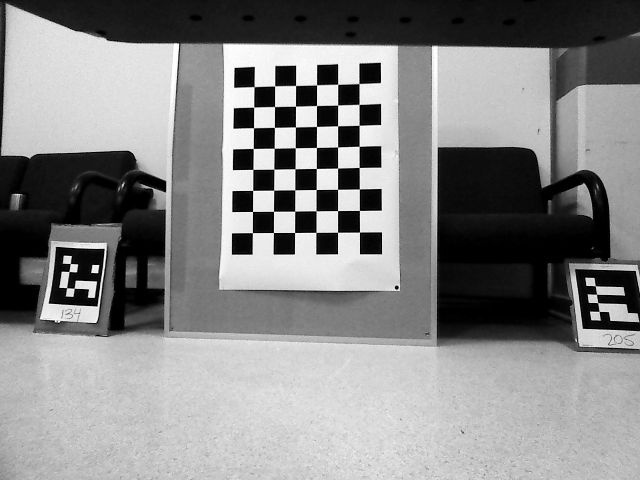
\includegraphics[width=0.5\linewidth]{calibration}
		\caption{Example of Calibration Image}
		\label{fig:calbcalbcalb}
	\end{figure}
	
	Large collections of images taken with calibration grids, like those shown in Figure \ref{fig:calbcalbcalb}, were used when running different tests of the camera. These image sets allowed for significantly quicker verification of all aspects of the camera.
	
	\subsection{Ground Based Robot}
	
	Testing the code on a ground based robot was necessary to ensure that the logic in the movement nodes is sound. Initial testing was done through simply having the robot follow moving targets or turn to face targets that are not head on. Initially simply watching the robot move away from obstacles was considered sufficient testing. When the project was sufficiently developed the testing was having the robot avoid obstacles and move towards a target. As the project moved closer to porting to the flying robot, the ground robot was tested to ensure it met the requirement outlined in the SOR \cite{sor}. 

	\subsection{Flying Robot}
	
	Due to time constraints along with difficulty in simply starting flying robots, this platform was not extensively tested for. 
	
	The cameras used in developing the monocular to depth vision were those mounted on the flying robots and the video collected was using these platforms. 

	
\section{Results - NOT DONE}

	- presentation of results
- prove we met the requirements

- we need to get some data points to prove the target and obstacles are found
- depth readings
- able to move towards the target? 
- talk about what happened with the obstacle avoidance and why it doesn't work


\subsection{Finding Targets}

\begin{figure}[H]
	\centering
	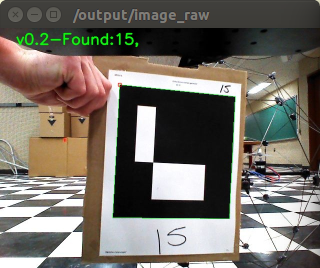
\includegraphics[width=0.45\linewidth]{resultsTarget}
	\caption{Positive Target Identification}
	\label{fig:targ}
\end{figure}

Finding targets, especially how they were defined, is fairly simple to perform by leveraging existing libraries. Every image that is published to the camera topic on by the robot is taken in and saved both in colour and in grayscale. The grayscale image is then passed into an ArUco searching library, which returns an array containing arrays which contain the id and corners of every marker discovered in the image.

Overlaying these corners on the colour image, as well as outputing the id number and any other necessary information was the easiest way to ensure that this program was discovering targets reliably. This frame is then published as its own image topic, an example of this output is shown in Figure \ref{fig:targ}.

\subsection{Extracting Depth Information}

\begin{figure}[H]
	\centering
	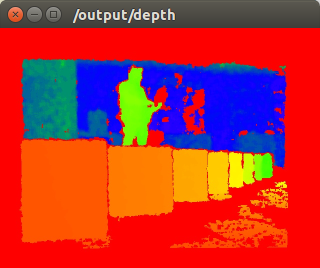
\includegraphics[width=0.45\linewidth]{verificationDepth}
	\caption{Registered Depth Image}
	\label{fig:deeeeeeeeeeeeeeeeeeeeeeeeeeeeeeeeeeeeeeeeeeeeeeeeeeeeeep}
\end{figure}

Extracting depth information, while using the TurtleBot, was done by using the depth registered images which use Astra Pro hardware to combine image information with depth information from a Lidar. This composite image can be coloured based on the depth values alone, and targets can be plotted on it for easy verification that samples are being taken from appropriate locations and interesting points. An example of the depth information is shown in Figure \ref{fig:deeeeeeeeeeeeeeeeeeeeeeeeeeeeeeeeeeeeeeeeeeeeeeeeeeeeeep}, which shows multiple boxes at different depths displaying an obvious gradient in colours.

\subsection{Compiling Odometry Information}

\subsection{Path Finding}


\section{Discussion}

\subsection{Overview}

	The design chosen is very capable of moving toward targets under control, and could even recognize, in the most abstract sense of the term, obstacles in its environment. Using a totally reactive approach felt overly simplistic, and is not interesting especially given the extremely small working space the lab provided.
	
	This caused the change in scope that resulted in this project not being ported to the flying robot. Instead of focusing on implementing an overly simplistic avoidance algorithm on an increasingly difficult platform to operate, the choice to build a greater memory into the program was made to allow for more complex obstacle avoidance.
	
	
\subsection{Flying Robot Requirements}

The majority of the requirements outlined are related to implementing code on a flying robot, so although there are existing solutions that have been verified to most of the requirements, the requirement that they be done on a flying robot leaves them not met.

Given that all of the solutions have been left highly portable, there is no software bound reason that the solution would not execute the same on board the flying robot, but the difficulty of operating a flying robot has prevented the project from to verifying that everything performs as expected.

\subsection{Major Issues}

The biggest issue for the entire duration of the project is the challenge of extracting depth information from a monocular camera. The flying robots only came with a monocular camera, and although initially it was intended to simply attach a second camera the decision to use this single camera was taken.

After a significant amount of time trying to parse depth information using OpenCV modules, it was discovered that it may be easier to use some sort of approach rooted in more modern machine learning algorithms. One of the most successful implementations discovered, which also provided all information needed to create custom models from relatively simple training sets, is Chaoyang Wang's approach.\cite{Wang_2018_CVPR} 

The machine learning approach did provide interesting results, but it has never been implemented into a depth module. The depth module simply uses the hardware registered depth information that is available from the TurtleBot's onboard sensors. These sensors did provide very accurate information, but are implemented later than useful simply to allow for the development of other modules, and would not be able to be ported over to the flying robot. 

Not having a verified manner to parse depth information that could be implemented on the flying robot left us wanting to push the driving platform to be able to perform more interesting obstacle avoidance.

\subsection{Recommendations for Future Expansion}

To expand further on this project, it would be necessary to find a testing environment that allows for more complex tests to take place. Even on the TurtleBot there are space limitations inside the lab to lay out obstacles in ways that could be navigated while still leaving far walls observable some of the time. 

Obtaining permission to test in a larger enclosed space would enable far more testing on both the ground and flying platforms at speeds where the models used may actually be able to produce useful results. 

The reactive and totally potential field based navigation is somewhat overkill when useful, and then when used with many obstacles and lower speeds became inadequate due to the way errors would accumulate.

The amcl approach is able to navigate quite complex environments, but would be useless in truly unknown environments or while moving at higher speeds. 

Using either the pushbroom algorithm or some other mechanism of sensing depth in the environment would result in a significantly more reliable system, and modeling more things as vectors against a central `odom' or `map' point would also prevent accumulating errors from causing as many problems as our earlier pfinder modules ran in to.
 
 \subsection{Functional and Performance Requirements}

	\begin{table}[H]
  \small
		\begin{tabular}{p{2cm} p{8cm} p{2cm} p{3cm}} 
			\hline
			{\textbf{Index}} & {\textbf{Description of Requirement}} & {\textbf{Result}} & {\textbf{Comment}} \\ \hline
FR-01 & The TurtleBot shall move towards a target under control & Met & \\
FR-02 & The TurtleBot shall recognize optically an OpenCV's ArUco shape and be able to give information on the location of the target relative to the robot & Met & \\
FR-03 & The TurtleBot shall recognize obstacles in its environment and identify where they are relative to itself & Met & Simply as areas that are occupied \\
FR-04 & The TurtleBot shall be able to make a deviation from its current movement pattern to avoid an obstacle in its path and then return to its pattern & Met & \\
FR-05 & The TurtleBot shall be able to identify multiple obstacles and avoid them accordingly & Partially Met & No concept of a particular obstacle, only points that are close \\
PR-01 & The TurtleBot shall be able to identify and locate OpenCV's ArUco shapes within a 15m radius & Met & \\ \hline
     \end{tabular}
     \caption{Summary of Results for the TurtleBot}
     \label{table:turtlbotresults}
 \end{table}

 The requirements for the TurtleBot can be seen in Table \ref{table:turtlbotresults}. The reason FR-04 was not satisfied on the TurtleBot is the same reason that was discussed in the results section. FR-05 also was not fully satisfied, the TurtleBot was able to recognize multiple obstacles at once and register each as a potential obstacle. The ability to avoid multiple obstacles, or to remember obstacles as objects based on having seen them multiple times from different angles, does not exist as the memory is too short term.

	\begin{table}[H]
  \small
		\begin{tabular}{p{2cm} p{8cm} p{2cm} p{3cm}}
			\hline
			{\textbf{Index}} & {\textbf{Description of Requirement}} & {\textbf{Result}} & {\textbf{Comment}} \\ \hline
FR-01 & The Flying Robot shall move towards a target under control & Not Met & Flying Robot was not Flown \\
FR-02 & The Flying Robot shall recognize optically an OpenCV's ArUco shape and be able to give information on the location of the target relative to the robot & Met & By subscribing to Flying Robots Camera Node\\
FR-03 & The Flying Robot shall recognize obstacles in its environment and identify where they are relative to itself & Not Met & Depth from single camera not verified\\
FR-04 & The Flying Robot shall be able to make a deviation from its current movement pattern to avoid an obstacle in its path and then return to its pattern & Not Met &  \\
FR-05 & The Flying Robot shall be able to identify multiple obstacles and avoid them accordingly & Not Met  &\\
PR-01 & The Flying Robot shall be able to identify and locate OpenCV's ArUco shapes within a 15m radius & Met & When processed off-board\\
PR-02 & The Flying Robot should be able to process an image and plot obstacles at a rate of 10 Hz & Met & When processed off-board \\
PR-03 & The Flying Robot shall be able to navigate an environment and detect up to two obstacles simultaneously & Not Met & \\ \hline
		\end{tabular}
		\caption{Summary of Results for the Flying Robot}
		\label{table:uavresults}
 \end{table}

Given that the flying robot was not implemented, most of these requirements are not met simply for the reason that it was not possible to verify if our solutions did work as expected on the flying robot.

 \subsection{Interface Requirements}

	\begin{table}[H]
  \small
		\begin{tabular}{p{2cm} p{8cm} p{2cm} p{3cm}}
			\hline
			{\textbf{Index}} & {\textbf{Description of Requirement}} & {\textbf{Result}} & {\textbf{Comment}} \\ \hline
IT-01 & The Gazebo simulator shall be run on a laptop and robots within the simulation will be interfaced through ROS & Met & \\
IT-02 & Communication to the TurtleBot will be done through ROS over USB & Met & \\
IT-03 & The Flying Robot will be communicating through ROS over WiFi wireless network & Met &\\
IT-04 & A simple interface, perhaps command line, will allow a user to select a marker as a target to start the robot's movement towards the target and this signal should be received over wireless transmission & Met & \\ \hline
		\end{tabular}
		\caption{Summary of Results for the Interface Requirements}
		\label{table:interresults}
 \end{table}
 
 \subsection{Simulation Requirements}

	\begin{table}[H]
  \small
		\begin{tabular}{p{2cm} p{8cm} p{2cm} p{3cm}}
			\hline
			{\textbf{Index}} & {\textbf{Description of Requirement}} & {\textbf{Result}} & {\textbf{Comment}} \\ \hline
SimR-01 & A Gazebo simulation environment which roughly approximates a lab environment with marker placed around will be created & Partially Met & Environments were created but not used\\
SimR-02 & Stationary obstacles will be added to the lab simulation environment and a TurtleBot shall navigate toward markers in the lab while avoiding obstacles & Not Met & \\
SimR-03 & An environment with obstacles will be created a Flying Robot shall navigate toward markers in the simulation while avoiding obstacles & Not Met & Flying Robot was never used in Gazebo \\ \hline
		\end{tabular}
		\caption{Summary of Results for the Simulation Requirements}
		\label{table:simresults}
 \end{table}

The use of simulation was limited due to the ease of operating the TurtleBot in the lab, combined with the ease of modifying the lab environment by simply moving boxes instead of having to make changes to the simulation environment.

 \subsection{Implementation Requirements}
 
	\begin{table}[H]
  \small
		\begin{tabular}{p{2cm} p{8cm} p{2cm} p{3cm}}
			\hline
			{\textbf{Index}} & {\textbf{Description of Requirement}} & {\textbf{Result}} & {\textbf{Comment}} \\ \hline 
ImpR-01 & OpenCV programs shall be created that can use a single video stream and identify both markers and obstacles & Met & \\ 
ImpR-02 & Prior to testing on the TurtleBot, the program shall be implemented on the gazebo simulation & Met & \\
ImpR-03 & Using the robot in the simulation environment the appropriate components, tools, and libraries to interpret and OpenCV stream, make decisions based on the environment, and execute instructions will be developed & Partially Met & Initial confirmation performed in Gazebo \\
ImpR-04 & The simplest obstacle avoidance algorithm must be implemented on a TurtleBot using ROS & Met & \\
ImpR-05 & The obstacle avoidance algorithm used for a Flying Robot will be implemented in a simulation & Not Met & \\ \hline
		\end{tabular}
		\caption{Summary of Results for the Implementation Requirements}
		\label{table:impresults}
 \end{table}

 
 \subsection{Schedule Requirements}

	\begin{table}[H]
  \small
		\begin{tabular}{p{2cm} p{8cm} p{2cm} p{3cm}}
			\hline
			{\textbf{Index}} & {\textbf{Description of Requirement}} & {\textbf{Result}} & {\textbf{Comment}} \\ \hline 
SchR-01 & The first TurtleBot simulation shall be able to operate in a Gazebo environment no later than November \nth{5} & Met & \\
SchR-02 & The first functional prototype shall be a TurtleBot robot capable of positively identifying a marker, moving towards the marker, and avoiding an obstacle placed in its environment no later than December \nth{18} & Met & \\
SchR-03 & The first functional prototype shall be capable of identifying a marker, moving towards the marker, and avoiding an obstacle placed in its environment no later than February \nth{18} & Met & \\
SchR-04 & Data Item Descriptions (DID) to be presented are DID-04: Preliminary Design Specification due November \nth{22}, DID-05: Preliminary Design Review Presentations due November \nth{29}, and the DID-06: Schedule Update is due January \nth{17}. The DID-07: Final Detailed Design Document is due March \nth{21}, the Final Project Presentation, DID-08, is March \nth{28} and the Final Project Demonstration, DID-09, is on April \nth{9} & Met & \\
& & & \\ \hline
		\end{tabular}
		\caption{Summary of Results for the Schedule Requirements}
		\label{table:schresults}
 \end{table}

\section{Conclusion}
The detailed design has been shown for Computer Optics for Analyzing Trajectories in Mostly Unknown, Navigation Denied Environments (\textsc{coatimunde}). The background outlined how the project progressed over the year and the motivation behind it. It provided a summary of the previous Data Item Deliverables, such as the Statement of Requirements and the Preliminary Design Document. The design section laid out the final design of the project and how it was implemented. The verification and validation section explained how different aspects of the project were tested throughout the year. The results section detailed the final results and how the requirements previously outlined were met. The discussion section gave a detailed analysis of the design in comparison with the requirements and made recommendations for future expansions of the project. The final design laid out in this document will also be used in the the Final Project Presentation and the Final Project Demonstration. 

\newpage
\printbibliography

\end{document}    
